%inputsP_POLDXrk_wALPHA_ItrqCLthoutputsP2_DX-1.tex

\begin{figure}[htbp]
	\centering 
	\subfloat[P2 DX: Narx identification]{
		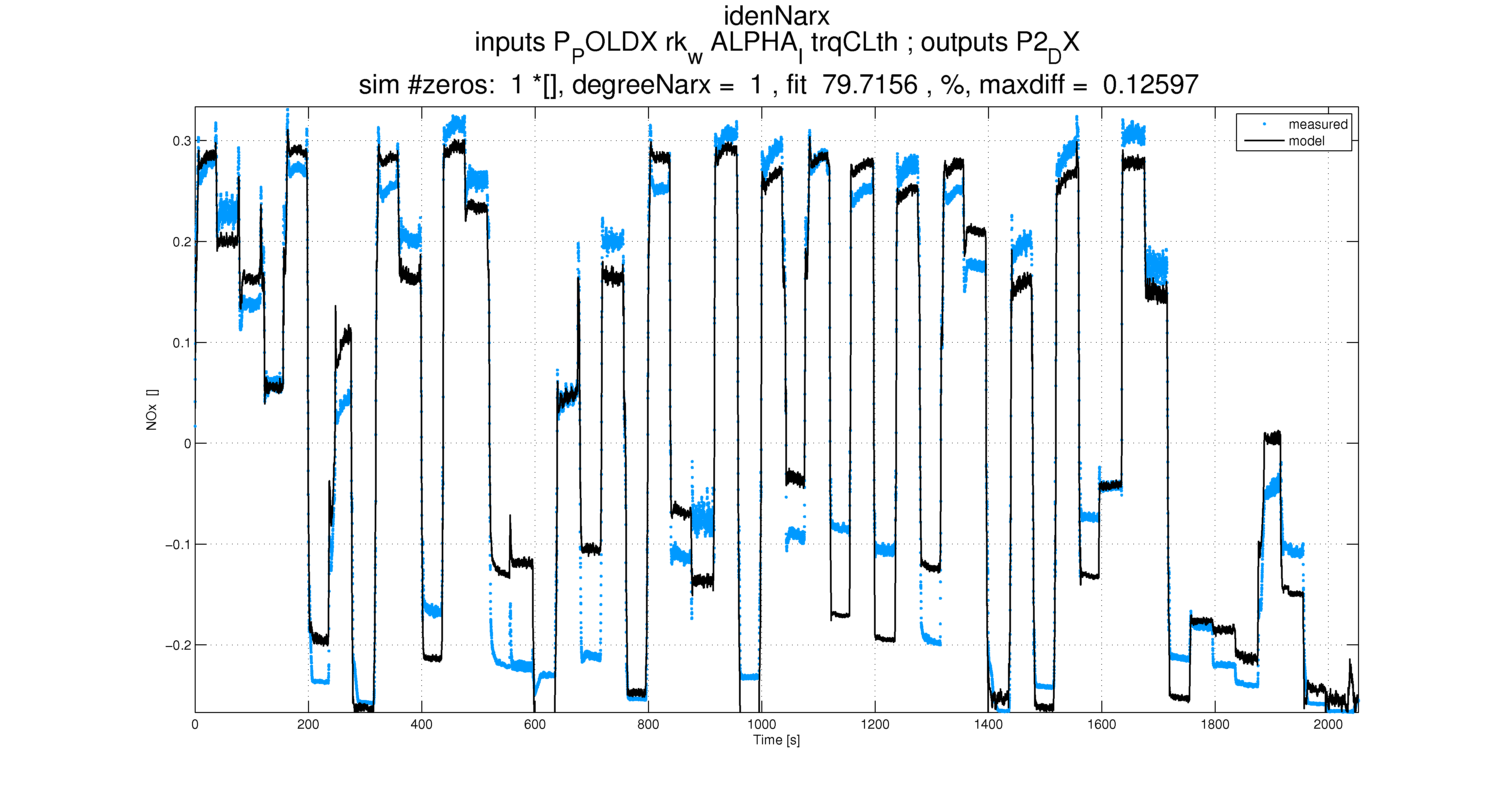
\includegraphics[width=.9\columnwidth]{Immagini/inputsP_POLDXrk_wALPHA_ItrqCLthoutputsP2_DX-idenNarx-1}
		\label{fig:inputsP_POLDXrk_wALPHA_ItrqCLthoutputsP2_DX-idenNarx-1}	}
	\\
	\subfloat[P2 DX: Narx prediction]{
		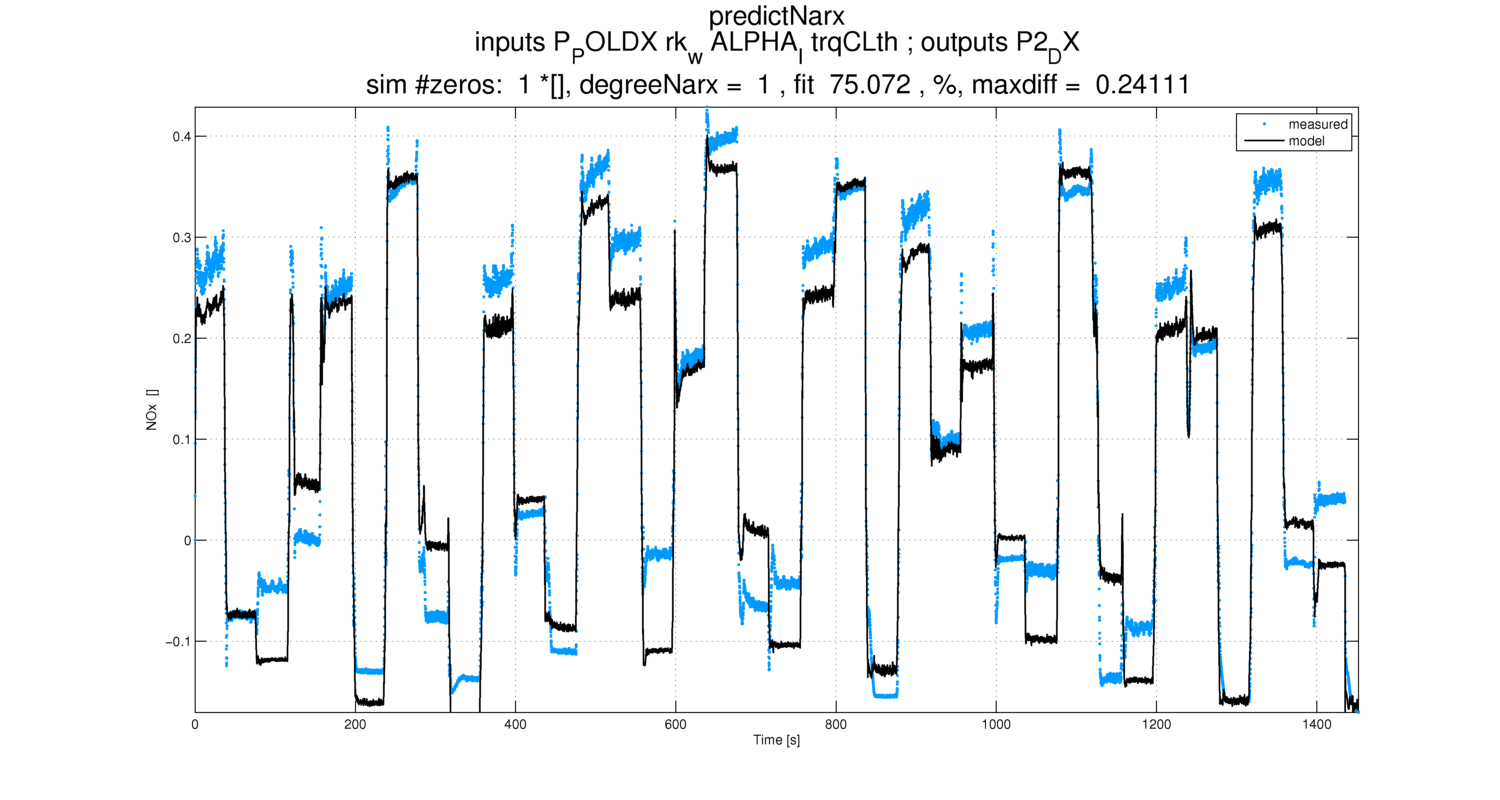
\includegraphics[width=.9\columnwidth]{Immagini/inputsP_POLDXrk_wALPHA_ItrqCLthoutputsP2_DX-predictNarx-1}
		\label{fig:inputsP_POLDXrk_wALPHA_ItrqCLthoutputsP2_DX-predictNarx-1}
	}
	\\
	\subfloat[P2 DX: Narx simulation]{
		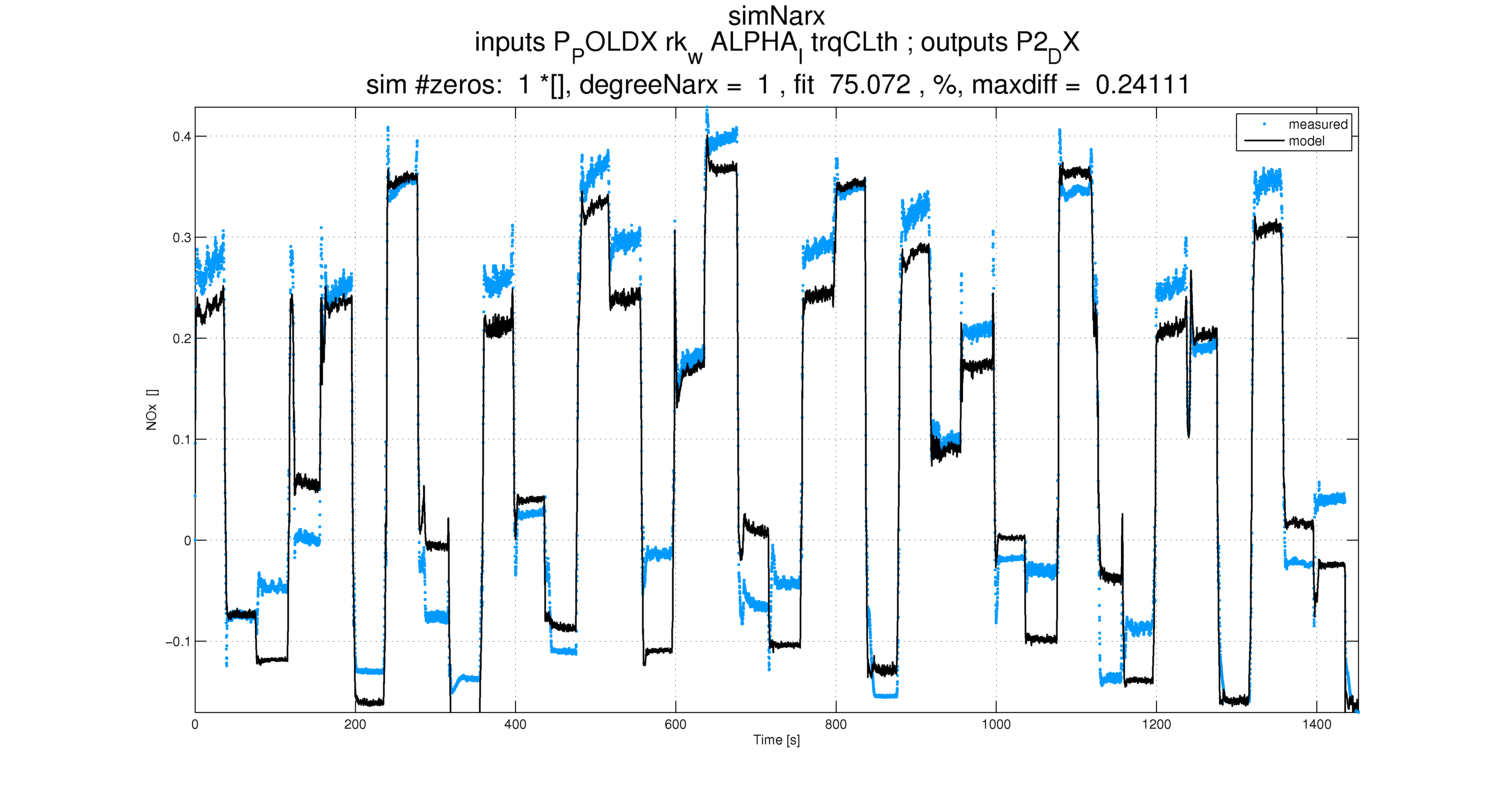
\includegraphics[width=.9\columnwidth]{Immagini/inputsP_POLDXrk_wALPHA_ItrqCLthoutputsP2_DX-simNarx-1}
		\label{fig:inputsP_POLDXrk_wALPHA_ItrqCLthoutputsP2_DX-simNarx-1}
	}
\phantomcaption
\end{figure}


\begin{figure}[htbp] \ContinuedFloat
	\centering 
	\subfloat[P2 DX: Transfer function identification]{
		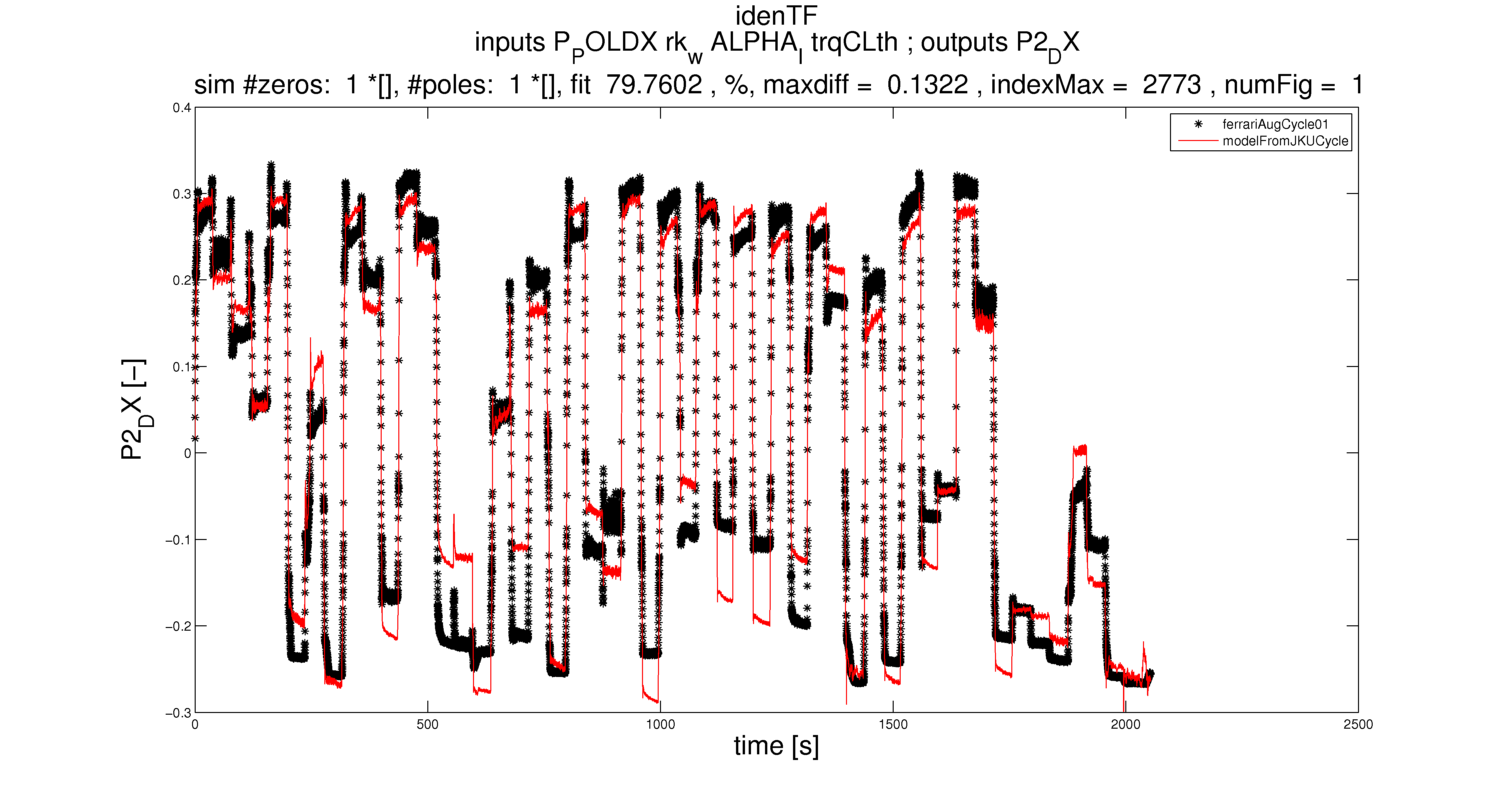
\includegraphics[width=.9\columnwidth]{Immagini/inputsP_POLDXrk_wALPHA_ItrqCLthoutputsP2_DX-idenTF-1}
		\label{fig:inputsP_POLDXrk_wALPHA_ItrqCLthoutputsP2_DX-idenTF-1}  }
	\\
	\subfloat[P2 DX: Transfer function simulation]{
		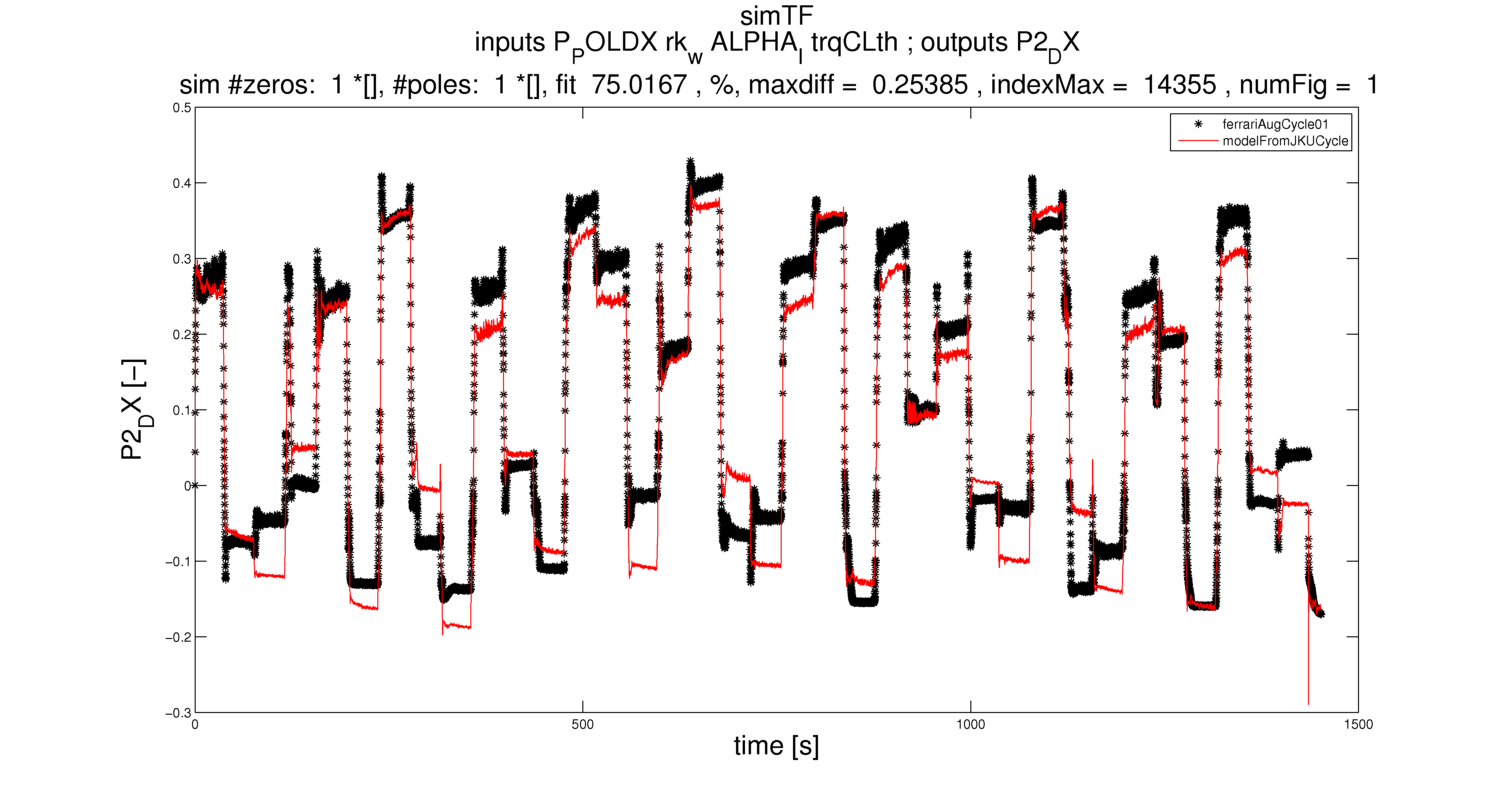
\includegraphics[width=.9\columnwidth]{Immagini/inputsP_POLDXrk_wALPHA_ItrqCLthoutputsP2_DX-simTF-1}
		\label{fig:inputsP_POLDXrk_wALPHA_ItrqCLthoutputsP2_DX-simTF-1}  }
	\\	
	\caption[Inputs: P POLDX, rk w, ALPHA I, trqCLth; Output: P2DX; np: 1; nz: 1; degree: 1]{Inputs: P POLDX, rk w, ALPHA I, trqCLth; Output: P2DX; np: 1; nz: 1; degree: 1}
	\label{fig:inputsP_POLDXrk_wALPHA_ItrqCLthoutputsP2_DX-1}
\end{figure}